\documentclass[pdftex,12pt,letter]{article}
\usepackage[margin=0.75in]{geometry}
\usepackage{verbatim}
\usepackage{graphicx}
\usepackage{xspace}
\usepackage{cite}
\usepackage{url}
\usepackage[pdftex,pdfpagelabels,bookmarks,hyperindex,hyperfigures]{hyperref}

\newcommand{\pd}{protoDUNE\xspace}
\newcommand{\xrd}{XRootD\xspace}

\title{The clustered storage option for the protoDUNE NP04 Online Buffer}
\date{\today}
\author{N. Benekos, M. Potekhin and B. Viren}


\begin{document}
\maketitle

\begin{abstract}
\noindent  This note describes the clustered storage
solution for the online buffer of the \pd (experiment NP04, Single-Phase LArTPC).
Basic data characteristics and  parameters of such storage are estimated. \xrd is proposed as the underlying
storage clustering technology. A portion of the existing   \textit{Neutrino Platform} computer cluster at CERN
can potentially be utilized for the development, testing and  implementation of the NP04 online buffer.  The reader
is encouraged to peruse  references to DUNE DocDB for more detailed information on individual
items included in this note.
\end{abstract}

%%%%%%%%%%%%%
\section{Overview}
\subsection{The online buffer}
The online buffer must be provided to absorb the potentially high instantaneous (in-spill) data rate before transmission
of data to mass storage and to satisfy the CERN requirement of providing 3 days worth of storage to make operation
of the experiment possible in case of a network and/or central services outage. Combined with the projected data
rate, this requirement determines the overall capacity of the buffer. From the buffer, the data needs to be delivered to
the disk storage (EOS) located at the CERN central services.
The place of the buffer in the data transmission chain therefore can be visualized as in Fig.\,\ref{fig:big-picture}.
\begin{figure}[tbh]
  \centering
  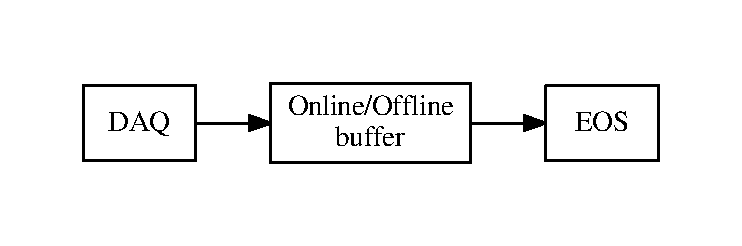
\includegraphics[width=0.7\textwidth]{figures/big-picture.pdf}
  \caption{Place of the buffer in the data transmission chain.}
  \label{fig:big-picture}
\end{figure}

\subsection{Data Characteristics}

The current ``data scenario'' estimates \cite{docdb1086} bracket the expected range of data rate
and data volume in \pd \cite{docdb186} due to in-spill beam triggers and out-of-spill cosmic ray muon triggers.
For historical reasons, the scenarios at the ends of this range are named ``Central'' and ``High rate''.

Two driving assumptions are the beam trigger rate and that one
cosmic-ray muon trigger is acquired out-of-spill for every in-spill
beam trigger.  Below is the summary of principal data characteristics:

\begin{description}
\item[trigger rate] 25 -- 50 Hz
\item[peak data rate (DAQ internal)] 1.5 -- 3.0 GByte/sec (instantaneous during spill)
\item[daily data volume] 25 -- 50TB
\item[3-day buffer capacity] 150 -- 300TB
\end{description}

\subsection{F-FTS}
Basic reqruirements for the system to handle the \pd raw data are presented in \cite{docdb1209}.
The design which meets these requirements is outlined in \cite{docdb1212}. It leverages the
Fermi File Transfer System (F-FTS) to perform two essential transfers:
\begin{itemize}
\item from the online buffer to CERN mass disk storage (EOS)
\item from EOS to CERN tape (CASTOR) and  mass storage at FNAL and other US sites
\end{itemize}

\noindent It is foreseen that two distinct instances of F-FTS will be deployed to fill each
respective role. This is schematically illustrated in Fig.\,\ref{fig:ftsinstances},

\begin{figure}[tbh]
  \centering
  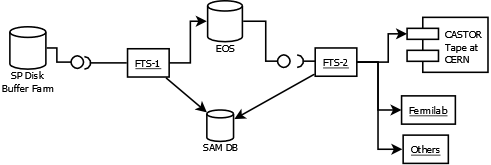
\includegraphics[width=0.7\textwidth]{figures/ftsinstances_v2.png}
  \caption{The two instances of FTS used for marshaling raw data from protoDUNE.}
  \label{fig:ftsinstances}
\end{figure}

 \noindent F-FTS uses the Fermilab SAM system for file catalog and metadata functionality,
and to keep track of the state of each transfer. In order to make use of this functionality, metadata
needs to be created before F-FTS takes ownership of a particular file. Checksums also need to be
generated to validate transfers throughout the chain of transmission. Computing the checksums
as well as collecting the necesary metadata require both I/O bandwidth and CPU.

Typically the F-FTS operates in the dropbox mode, whereby it detects the arrival of a new file
according to configurable rules. It must therefore have a POSIX-like access to the file
system which is under its watch. Alternatively, F-FTS can be triggered via a HTTP request
from an external agent. The actual transfer can be handled by F-FTS itself (i.e. it works
as a client) or by third-party tools.

\section{The online buffer}
\subsection{Attached vs Clustered Storage}
Any data taking scenario currently under consideration requires sustained rate
of data to disk in hundreds of MB per second. In practice this means that
multiple hard drives are needed to absorb such rate and have enough headroom
for stable operation of the system.



\section{Concept}

The \texttt{neut} cluster is now being formed using some 300 nodes in
total reclaimed from ATLAS.  We will dedicate about 50 nodes in
support of developing the disk buffer system for the single-phase
protoDUNE detector adequately scaled for storing three days worth of
expected data.  To label this sub-cluster we say
``\texttt{neut-spbuf}''.  Initially \texttt{neut-spbuf} will be for
developing and testing the buffer system design.  Meanwhile, we will
explore what is needed to migrate \texttt{neut-spbuf} into actual
operation.

\section{Disk}

The current \texttt{neut} nodes have very limited disk storage.  The
\texttt{neut-spbuf} nodes must be upgraded to provide storage to meet
the 3-day buffer requirement. To meet the ``High rate'' requirement we
will install $2\times 3$TB SATA disks in each of the 50
\texttt{neut-spbuf} nodes.

\section{Networking}

The ``High rate'' scenario requires sinking a peak of 3.0 GByte/sec
(24 Gbps) throughput during the beam spill.  Between spills, when
cosmic muon triggers are acquired, the throughput is somewhat reduced
but we take 3.0 GByte/sec as our requirement.  Spread across the 50
\texttt{neut-spbuf} nodes these streams this will approximately fill
50\% of the existing 1Gbps NICs.  We expect similar multiplicity at
the data production end (the Event Builder layer of the pD/SP DAQ).

During initial testing we will request a 20 Gbps link between the
current location of \texttt{neut}\footnote{CERN building 185} and
central CERN computing including EOS and the pD/SP detector
site\footnote{CERN building EHN1}.

To supply this connectivity we require 50 switch ports at 1Gbps and
(effectively) one switch port at 20Gbps.  Based on our current design
it is possible to segment the network streams so that the total
bandwidth is spread over multiple switches, for example two switches
each with 25 ports at 1Gbps and 1 port with 10 Gbps.  One example
switch is the Cisco SG500X-48P which can provide 48 1Gbps ports and
ample ports on the high-bandwidth side.  One such switch is needed on
the DAQ end of the 20Gbps link and one on the \texttt{neut-spbuf} end.

\begin{thebibliography}{1}
\bibitem{docdb1086}
{DUNE DocDB 1086: \textit{ protoDUNE/SP data scenarios with full stream (spreadsheet)}}\\
\url{http://docs.dunescience.org:8080/cgi-bin/ShowDocument?docid=1086}

\bibitem{docdb186}
{DUNE DocDB 186: \textit{ ProtoDUNE Proposal}}\\
\url{http://docs.dunescience.org:8080/cgi-bin/ShowDocument?docid=186}


\bibitem{docdb1209}
{DUNE DocDB 1209: \textit{Basic Requirements for the protoDUNE Raw Data Mangement System}}\\
\url{http://docs.dunescience.org:8080/cgi-bin/ShowDocument?docid=1209}


\bibitem{docdb1212}
{DUNE DocDB 1212: \textit{Design of the Data Management System for the protoDUNE Experiment}}\\
\url{http://docs.dunescience.org:8080/cgi-bin/ShowDocument?docid=1212}



\bibitem{xrootd}
{XRootD, high performance, scalable fault tolerant access to data  repositories}.\\
  \url{http://xrootd.org/}.

\end{thebibliography}


\end{document}

%%% Local Variables:
%%% mode: latex
%%% TeX-master: t
%%% End:
